\documentclass[12pt,a4paper]{amsart}

\usepackage[slovene]{babel}
\usepackage[utf8]{inputenc}
\usepackage{amsmath,amssymb,amsfonts,bm}
\usepackage{url}
\usepackage{graphicx,subfig}


\textwidth 15cm
\textheight 24cm
\oddsidemargin.5cm
\evensidemargin.5cm
\topmargin-5mm
\addtolength{\footskip}{10pt}
\pagestyle{plain}
\overfullrule=15pt

%%%%%%%%%%%%%%%%%%%%%%%%%%%%%%%%%

%Naslovnica%
\begin{document}
    
\thispagestyle{empty}
\noindent{\large
Univerza v Ljubljani\\[1mm]
Fakulteta za matematiko in fiziko\\[3mm]
Finančna matematika -- 1.~stopnja}
\vfill

\begin{center}{\large
Urška Komatar, Ian Lampič\\[2mm]
{\Huge \bf Intransitive dice}\\[5mm]
Projekt pri predmetu Finančni praktikum\\[1cm]}
\end{center}
\vfill

\noindent{\large
Ljubljana, 2023}
\pagebreak

\tableofcontents
\pagebreak


\section{Predstavitev osnovnega problema}
\subsection{Problem}
Naj bo $p > \frac{1}{2}$ konstanta, A, B in C pa 6 - strane kocke z različnimi števili na svojih straneh, tako da kocka A premaga
B z verjetnostjo vsaj $p$, B premaga C z verjetnostjo vsaj $p$ in C premaga A z verjetnostjo vsaj $p$. Želimo poiskati maksimalni $p$ tako, 
da bo obstajala trojica kock, za katere bo veljala dana lastnost. Kasneje si bova ogledala še primere s štirimi kockami, trostranimi kockami, štiristranimi kockami
in kockami s petimi stranmi.

\subsection{Ideja reševanja}
Najprej bova sestavila pomožno funkcijo, ki bo za argumente prejela seznam treh seznamov. V vsakem seznamu bo 6 naravnih števil, ki bodo predstavljale števila na kocki. Če so A, B in C slučajne spremenljivke, ki povedo, koliko pokaže posamezna kocka, bo torej funkcija vračala $min(P(A>B), P(B>C), P(C>A))$. Nato bi naredila krovno funkcijo, ki bi sprejela
naravno število $n$. Znotraj te funkcije bi generirala seznam seznamov z elementi prvih $n$ naravnih števil in na vsakem takem seznamu poklicala pomožno funkcijo.
Medtem bi beležila dobljene verjetnosti in na koncu vrnila maksimum teh vrednosti. Za vsa nadaljna vprašanja bova funkcijo prilagodila danim zahtevam in ponovila postopek.

\subsection{Primeri netranzitivnih kock}

\subsubsection{Primer}
\begin{itemize}
    \item A: 2, 2, 6, 6, 7, 7
    \item B: 1, 1, 5, 5, 9, 9
    \item C: 3, 3, 4, 4, 8, 8
\end{itemize}
\begin{align*}
    P(A > B) = P(B > C) = P(C > A) = \frac{5}{9}
\end{align*}
\\Primer, ko je $p=\frac{5}{9}$

\subsubsection{Efronove kocke}
Efronove kocke so set štirih netranzitivnih kock A, B, C in D z naslednjimi številkami na stranicah:
\begin{itemize}
    \item A: 4, 4, 4, 4, 0, 0
    \item B: 3, 3, 3, 3, 3, 3
    \item C: 6, 6, 2, 2, 2, 2
    \item D: 5, 5, 5, 1, 1, 1
\end{itemize}
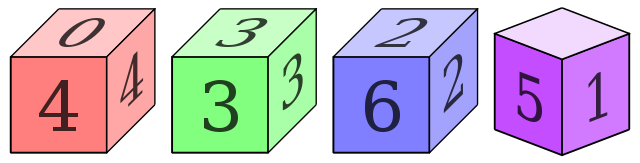
\includegraphics[width=100mm]{Efron's dice.png}
\\Vsaka kocka je premagana s prejšnjo z verjetnostjo $\frac{2}{3}$:
\begin{align*}
   P(A>B) = P(B>C) = P(C>D) = P(D>A) = \frac{2}{3}
\end{align*}
 
B ima na vseh straneh enako število (B je konstantna). A ima 4 od 6 števil višja od B, torej verjetnost da A premaga B je $\frac{2}{3}$, medtem ko
C pa ima 4 od 6 števil manjša od B, torej B premaga C z verjetnostjo $\frac{2}{3}$.
\\$P(C>D)$ izračunamo s seštevanjem pogojnih verjetnosti:
\begin{itemize}
    \item C pokaže 6 ($P = \frac{1}{3}$); premaga D z verjetnostjo 1
    \item C pokaže 2 ($P = \frac{2}{3}$); premaga D le, če D pokaže 1 ($P = \frac{1}{2}$)
\end{itemize}

Torej verjetnost da C premaga D je naslednja:
\begin{align*}
    (\frac{1}{3}\cdot 1)+(\frac{2}{3}\cdot\frac{1}{2}) = \frac{2}{3}
\end{align*}

S podobnim izračunom dobimo še verjetnost, da D premaga A.


\section{Reševanje osnovnega problema}
\subsection{Primerjava kock}
V prvem koraku sva naredila funkcijo $comparison$, ki \linebreak
sprejme dva seznama, ju uredi po naraščajočem vrstnem redu in prešteje, koliko števil prvega seznama je večjih od števil iz drugega seznama. Nato ta števila shrani že 
v prej definiran prazen seznam in vrne ta seznam kot rezultat.
Seznama nam predstavljata dve kocki, števila v njih pa so števila na stranicah kock.
 \begin{verbatim}
    def comparison(lst1, lst2):
    count = 0
    p = []
    lst1.sort()
    lst2.sort()
    for i in range(len(lst1)):
        for j in range(len(lst2)):
            if lst1[i] > lst2[j]:
        count = 0 
    return p
 \end{verbatim}
 \subsection{Intranzitivnost}
 V naslednjem delu sva naredila funkcijo $intransitive$, ki za argument prejme seznam seznamov, kar predstavlja dane kocke.
 Nato se na danih kockah izvede funkcija $comparison$, v prej definiran prazen seznam pa se shranjujejo vsote seznamov, ki jih ta funkcija vrne.
 Na koncu vzame minimum vseh vsot, kar predstavlja verjetnost, da med danimi kockami ne velja tranzitivnost. Funkcija vrne to verjetnost in pa kocke, ki jim ta verjetnost pripada.
 \begin{verbatim}
    def intransitive(dice):
    numb_of_dice = len(dice)
    lst_of_probs = []
    for i in range(numb_of_dice - 1):
        comparison(dice[i], dice[i+1])
        lst_of_probs.append((sorted(dice[i]), sorted(dice[i + 1]),
         sum(comparison(dice[i], dice[i+1]))))
    lst_of_probs.append((sorted(dice[numb_of_dice-1]), 
    sorted(dice[0]), sum(comparison(dice[numb_of_dice-1], dice[0]))))
    prob = 100 #določena zgornja meja za minimum, ki ne bo presežena
    for i in range(len(lst_of_probs)):
        prob = min(prob, lst_of_probs[i][2])
    return prob, dice
 \end{verbatim}

 \subsection{Generator kocke}
 Naslednja funkcija naredi seznam različnih naravnih števil, ki jih bo izbrala slučajno na intervalu $\left[1,m\right]$. 
 Število elementov seznama je enako številu stranic kocke, kar pa predstavlja argument $sides$.
 \begin{verbatim}
    def generator_list(m, sides):
    st = set()
    while len(st) < sides:
        random_num = random.randint(1, m)
        st.add(random_num)
    return list(st)
 \end{verbatim}

 \subsection{Krovna funkcija}
 Krovna funkcija $m$-krat naredi $num\_of\_dice$ kock in v prej definiran prazen seznam shranjuje rezultate funkcije $intransitive$. 
 Generator, ki nam generira dane kocke za argument sprejme $n$, kar predstavlja zgornjo mejo intervala, iz katerega izbira naravna števila in pa število kock, kar pa predstavlja argumentom $sides$.
 Na koncu izmed vseh rezultatov novega seznama vrne maksimum, kar predstavlja največjo verjetnost, da med danimi kockami ne velja tranzitivnost, izmed vseh različnih kombinacij kock v tem seznamu.
 Funkcija vrne to verjetnost in pa kocke, ki jim ta verjetnost pripada.
\begin{verbatim}
    def krovna(n, m, sides, num_of_dice):  
    lst = []
    while len(lst) < m: 
        dice = []
        for i in range(num_of_dice):
            dice.append(generator_list(n, sides))
        lst.append(intransitive(dice))
    max_prob = 0
    for i in range(len(lst)):
        if max_prob < lst[i][0]:
            max_prob = lst[i][0]
            lst_with_max = lst[i][1]
    return max_prob, lst_with_max
 \end{verbatim}
 \pagebreak
 \section{Rezultati}

 \subsection{Rezultati v odvisnosti od k-stranosti}
 \begin{center}
    \includegraphics*[width=120mm]{st_stranic.png}
 \end{center}
 Graf predstavlja spreminjanje verjetnosti v odvisnosti od števila stranic. V vseh primerih smo poskus ponovili s tremi kockami. Opazimo, da je maksimum funkcije v primeru, ko imamo 5-strane kocke. V nobenem primeru ne presežemo verjetnosti 0.6, kar je tudi zgornja meja za dani problem.
 
 \subsection{Rezultati v odvisnosti od števila kock}
\begin{center}
    \includegraphics*[width=120mm]{st_kock.png}
\end{center}
V zgornjem grafu je prikazano, kako število kock vpliva na verjetnost, da za dane kocke ne velja tranzitivnost. V poskusu sva uporabila 3-strane kocke. Ugotovila sva, da verjetnost s povečanjem števila kock počasi pada.

\subsection{Opomba rezultatom}
Za vsak komplet kock sva eksperiment ponovila 2,5 milijonkrat, torej lahko sklepamo zaradi velikega števila ponovitev, da so rešitve zelo blizu pravim, vseeno pa lahko pričakujemo pri kakšnem primeru manjše odstopanje zaradi omejenosti števila ponovitev. Za večjo zanesljivost sva rezultata za primer s tremi in štirimi 6-stranimi kockami preverila tudi pri drugih virih in ugotovila, da se ujemajo z najinimi rešitvami.
%%%%%%%%%%%%%%%%%%%%%%%%%%%%%%%%%%%%%%%%
\end{document}